\section{Problems}

\begin{questions}
\question{Solve the Huggett economy using the endogenous grid method}
\begin{solution}

Here is a link to my code: \url{https://github.com/filipmellgren/QMM/tree/main/ps3}.

Again, I leaned heavily on Python, Numpy, and Numba to solve the problem set.

The path for interest transition that I find is as follows:

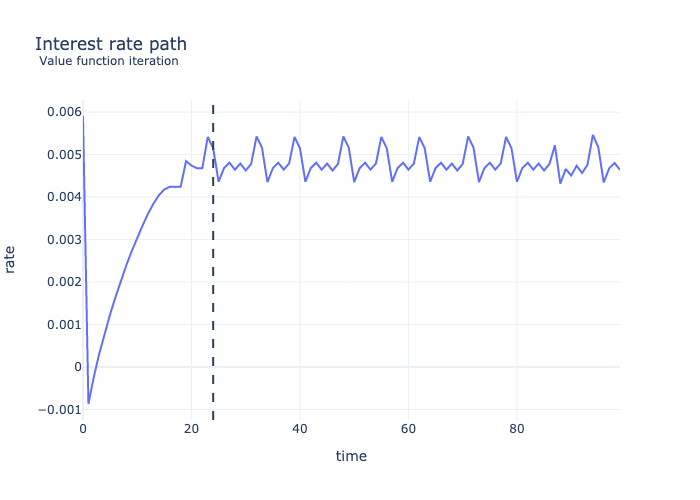
\includegraphics[scale=0.5]{figures/rate_path.png}

It is surprising to see that the final interest rate is actually lower than the initial interest rate, which suggests yet another bug in the code. Nontheless, this week saw a major overhaul of the code I used in PS2 and I think I made good progress and caught some bugs. 

I managed to implement the endogenous grid method and it now gives me a policy that is very similar to that of the value function iteration. The two won't correspond exactly due to the discrete grid, after projecting the endogenous choices onto the exogenous grid, some differences remain but they often overlap.

I did not have time and energy to reproduce the distribution over welfare gains this week, I spent a lot of time on the main functionality, implementing the EGM, and tracking bugs from last week's problem set.

\end{solution}
\end{questions}


